% !TEX root = ../foresight.tex

\section{Introduction}

% \ja{Add reference to all figures, tables and algorithms in the text.}

% <<<<<<< HEAD
% \begin{figure}
%     \centering
%
%     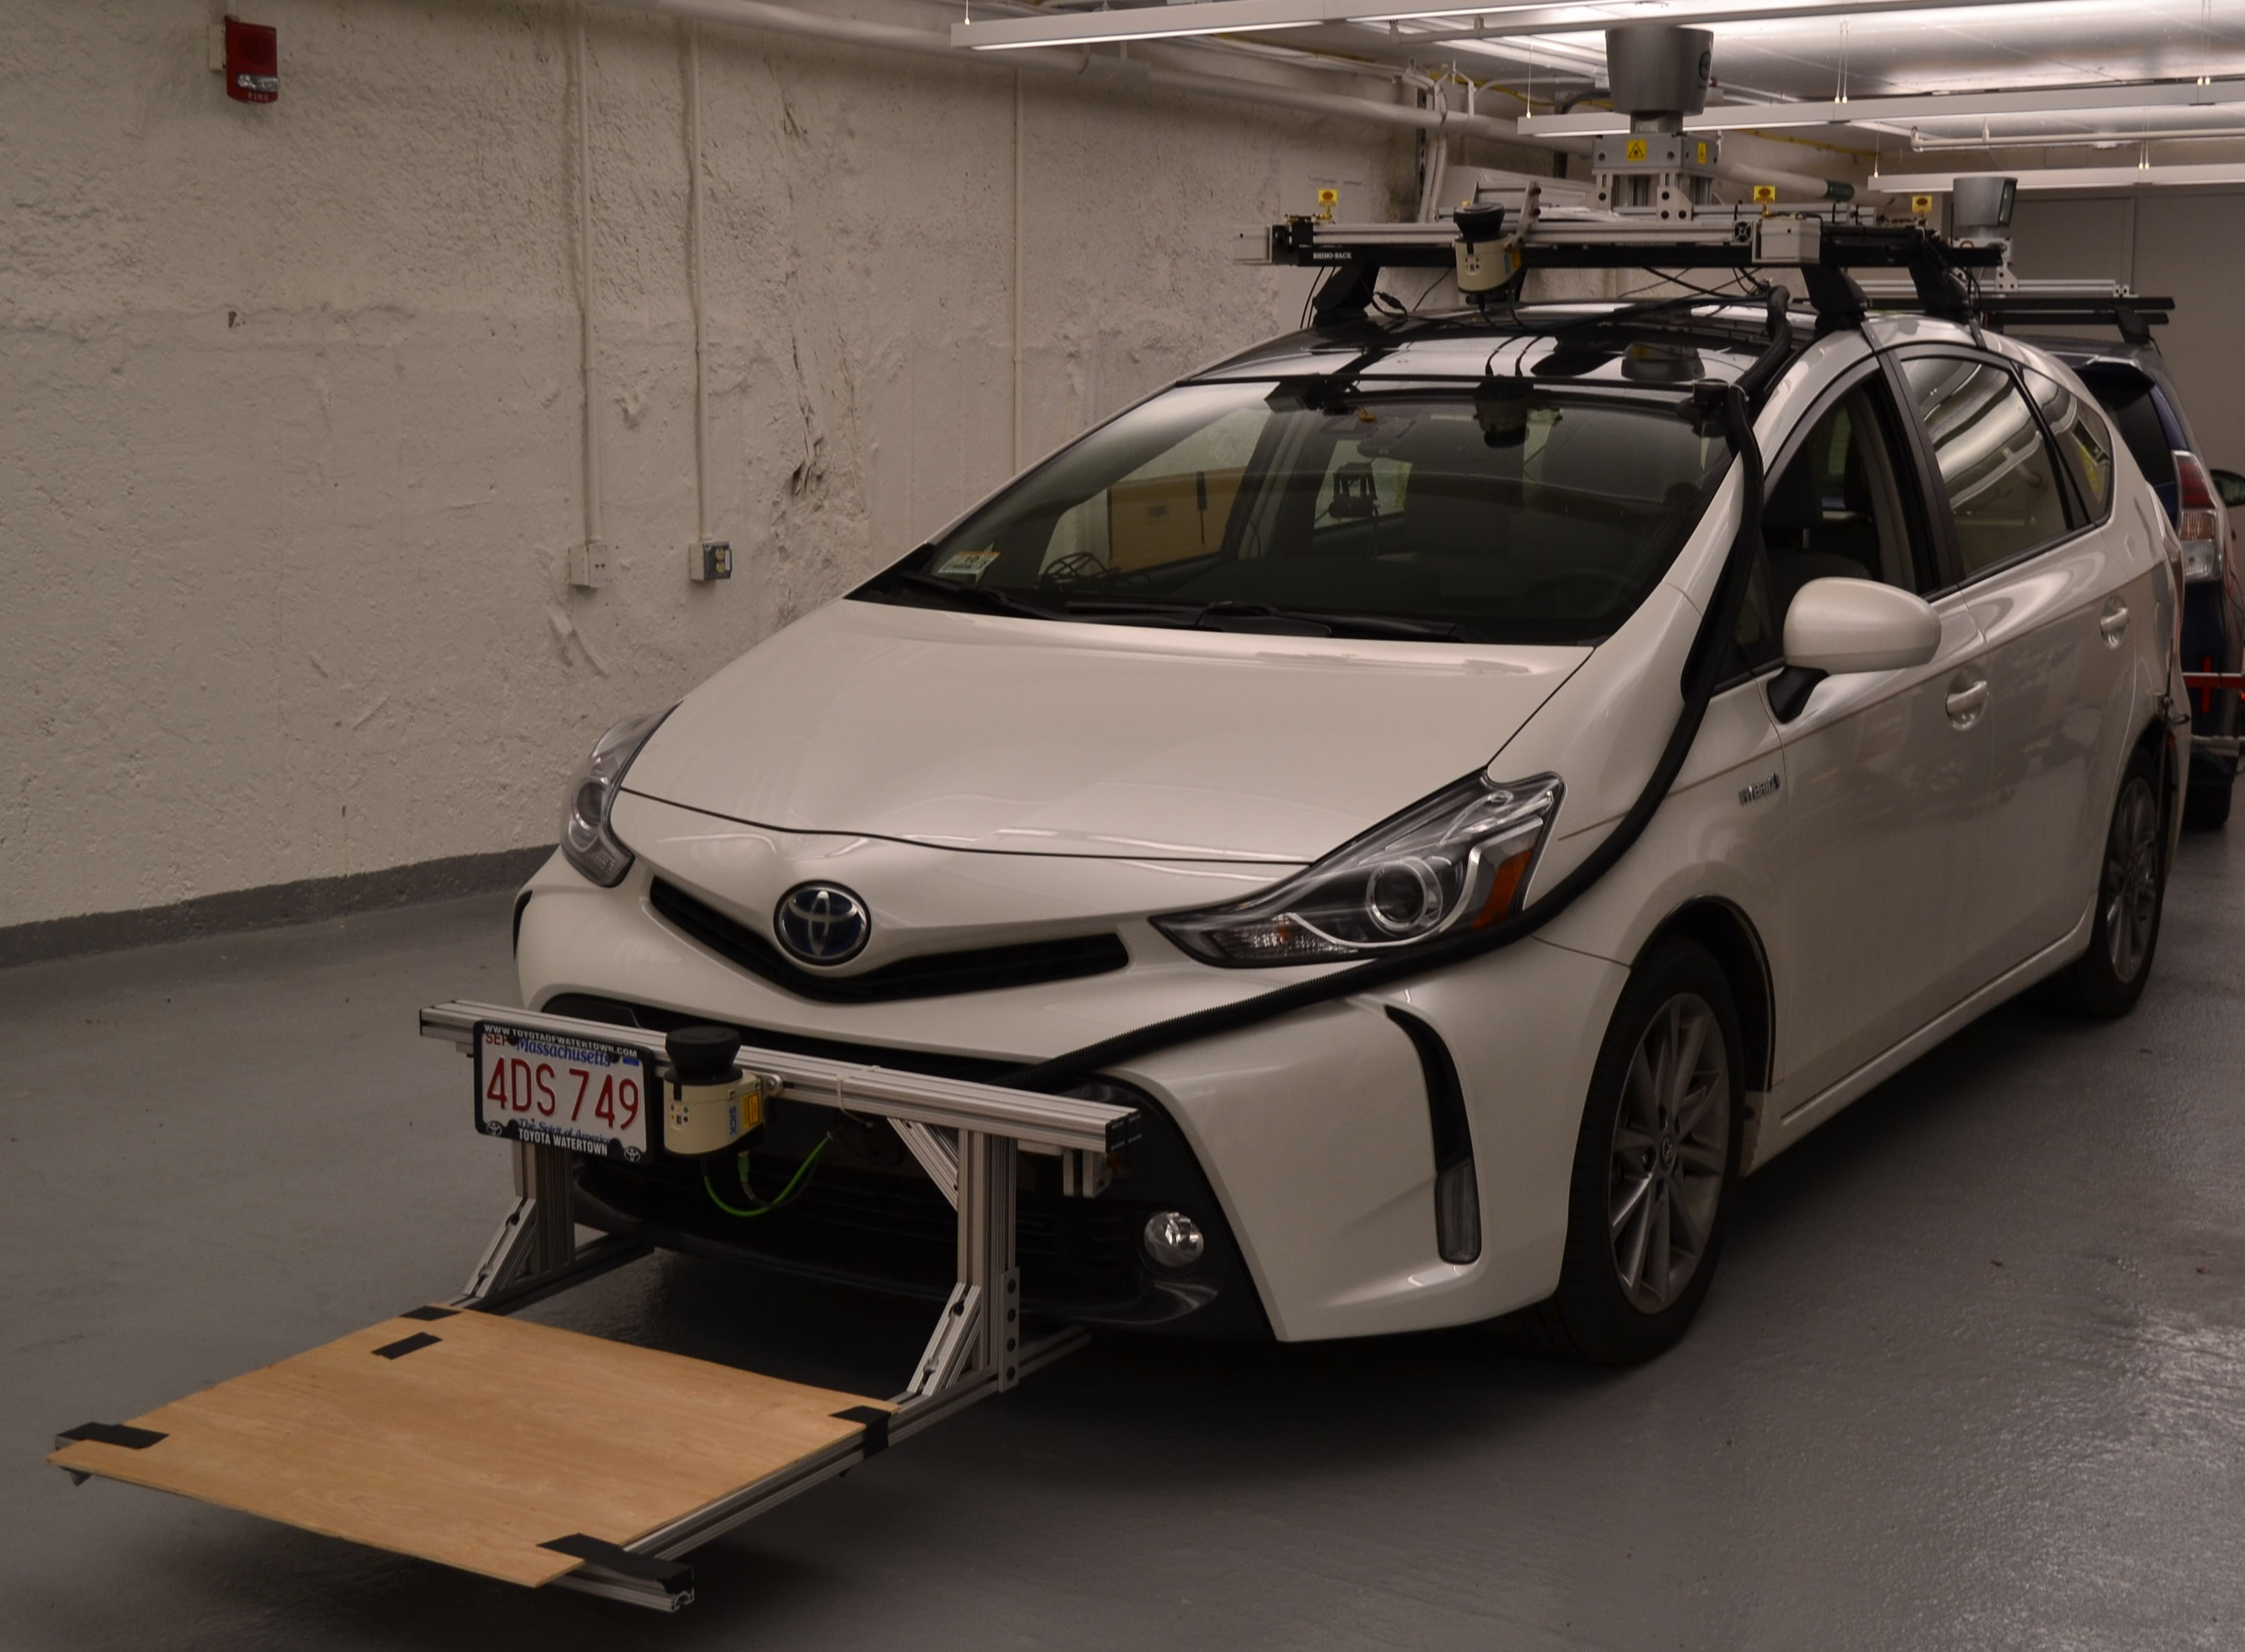
\includegraphics[angle=90, width=0.6\linewidth]{car}
%
% \end{figure}

Globally, over 3000 people lose their lives in vehicle-related accidents and over one hundred thousand are injured or disabled on average \emph{every day} \cite{ASIR2016}.
% Worse still is that this number is continuing to increase \cite{NSC2016Fatality}.
In the United States, over 90\% of these accidents are due to human error \cite{NHTSA_crash_stats}.
This has resulted in the continued development of advanced safety systems by commercial car manufacturers.
%Safety systems in automobiles are undergoing rapid development to address the fact troubling continued increase in traffic injuries and fatalities \cite{NSC2016Fatality}. 
For example, systems exist to automatically brake in the case of unexpected obstacles \cite{Toyota_patent}, maintain a car in a lane at a given speed \cite{bradley2016tesla}, and alert users of pedestrians, signage, and other vehicles on the roadway \cite{Dagan_IVS_2004}. These systems will make our cars safer and eventually autonomous.
However, many accidents are due to blind spots, for example when a vehicle takes a turn with poor visibility or when a pedestrian crosses from behind a parked vehicle. In these accidents, vulnerable road users, i.e. pedestrians and bikers, are typically involved and the consequences are dramatic.

We propose to extend the perception capabilities of a vehicle, autonomous or human-driven, with a small Unmanned Aerial Vehicle (UAV) capable of taking off from the car, flying around corners to gather additional data from blind spots and landing back on the car after a mission. Small UAVs are highly mobile and agile, and they are capable of capturing aerial footage autonomously\cite{naegeli17letters}.
The quadcopter could use the car as a charging base,
while the car could send the quadcopter out on missions to scout ahead and
fill in the blind spots in its vision.

A crucial step in enabling a small UAV and an autonomous car to work
together is to ensure that there exists an accurate pose transform between the car
and the quadcopter. In
this paper, we present a method for relative localization using ultra-wideband
radios (UWBs) to measure the relative position of the quadcopter relative to the car
with an accuracy of less than 14cm. This information is fused with the internal
state estimation to enable the UAV to safely navigate to blind spots and then
land back on the car. Furthermore, we have developed a path planning algorithm
for remote sensing and have carried out experiments using a quadrotor and a
car.

% The accuracy of GPS is not sufficient when the UAV must navigate
% obstacle-filled environments (such as a city center) or land on the car.

%implemented a Deep Neural Network to detect obstacles, such as pedestrians, from the UAV.
% In addition, we have implemented a real-time obstacle detection system, useful for detecting pedestrians from the UAV, using a deep neural network system called YOLO \cite{darknet}. The YOLO neural network divides the image into regions, and predicts the probability and object type for each region that is proposed to be an obstacle. Its unique detection method allows it to run at 15 FPS on our GPU-enabled system, much faster than other approaches.

%Introduction: Lots of accidents due to not seeing what's going on. For example a pedestrian or a biker behind a car. Could be similar to the motivation in Wilko's paper.
%
%Autonomous systems are becoming increasingly integrated into
%our daily lives. Two of the most conspicuous examples are UAVs,
%which are used to capture aerial footage, and autonomous cars,
%which promise to make driving much safer and more convenient
%than it is today. Unfortunately, both of these types of autonomous
%robot have deficiencies. UAVs are highly mobile and agile, but they
%have limited range and payload capabilities. Meanwhile, cars and trucks
%have range and payload capabilities several orders of magnitude greater than
%those of UAVs but, being constrained to traveling on roads, are far less mobile.
%
%In the context of autonomous cars, this mobility constraint becomes apparent
%when navigating corners and crowded environments. Since a car cannot
%see around corners and other obstacles without physically reorienting its
%entire bulk, it must often navigate with little information about what obstacles
%it may encounter. Therefore it is blind to obstacles such as a biker or little old
%lady crossing the street behind an oncoming bus and therefore must proceed
%with extreme caution. Pairing an autonomous car with a quadcopter is a potential
%solution to this problem - the quadcopter could use the car as a charging base,
%while the car could send the quadcopter out on missions to scout ahead and
%fill in the blind spots in its vision.
%
%The one crucial step in enabling a quadcopter and an autonomous car to work
%together is to ensure that there exists an accurate transform between the car
%and the quadcopter. GPS, which has an accuracy of about +/- 2m, can suffice
%for when the quadcopter is navigating broad open spaces. However, +/- 2m
%accuracy is completely insufficient for when the quadcopter must navigate
%obstacle-filled environments (such as a city center) or land on the car. In this 
%paper, we present a method using ultra-wideband radios to measure the relative 
%position of the quadcopter relative to the car with +/- 10cm accuracy, enabling 
%the quadcopter to safely navigate to blind spots and then land back on the car.


%\subsection{Related works}

%Motion planning for autonomous cars. Some methods assume full knowledge of the environment [] -> not realistic, while others [] only have local sensing. Our method would work in parallel and provide a "better" map.

Our method has similarities with multi-robot mapping. For instance \cite{Michael:2012gl} and \cite{Forster:2013kn} combined the maps from a ground and an aerial robot for enhanced exploration and \cite{Delmerico:2017vq} employed a map created by an aerial robot for planning the motion of a ground robot. % There has also been some preliminary work in \cite{nasser2015fleye} that tackled the communication problems associated with flying a quadrotor with a ground vehicle; however, it did not look into the planning and perception needed to provide useful information to the ground vehicle.

%Our method explores the frontiers of the map built by the ground robot and is similar to exploration \cite{}. Our idea is similar, yet we focus on the context of safe autonomous driving in cluttered urban environments.


Quadrotors have been able to track a moving vehicle using visual techniques
such as AprilTag localization \cite{borowczyk2016autonomous}, optical flow \cite{herisse2012landing},
and infrared markers \cite{wenzel2011automatic}. However, a weakness of visual systems
is that visual cues must be in the line
of sight of the quadrotor-mounted camera. Moreover, the lighting conditions must be suitable
for the cameras. These restrictions limit the usefulness of visual tracking. Meanwhile,
GPS tracking, while useful in long-range outdoors scenarios, is not accurate enough for 
maneuvers such as landing and obstacle avoidance. For example, average accuracy in
smartphone GPS receivers is 4.9 m \cite{gpsaccuracy}.

UWB sensors have in recent years become a popular tool for
localization of quadrotors, particularly in indoor GPS-denied environments 
\cite{liu2007survey, prorok2014, hollinger2012target}, since they can
provide distance measurements with an accuracy of 10 cm and a range of
up to 300 m\cite{Decawave_Website}. Indoor localization of quadrotors has been
achieved by placing UWB ``anchors" around the perimeter of a room and attaching
a UWB ``tag" on the quadrotor.  Using this technique, \cite{mueller2015fusing}
and \cite{kempke2016harmonium} have achieved localization with accuracy on the order
of 30cm.

The problem of relative localization is more challenging because the UWB tag is outside of
the perimeter of the anchors. However, in \cite{tobiuwb}, a quadrotor
outfitted with four UWBs was able to follow a person carrying a UWB tag
in the plane of the quadrotor
with less than 10 cm mean error. The authors achieved this accuracy using an
iterated Extended Kalman Filter. Building off of this work, we used
6 UWB sensors on a car to estimate the 3D position of a UWB on a quadrotor with an
average mean error of 13.7 cm. Moreover, unlike in previous systems,
we take advantage of the accurate relative transform to use the sensors
on the car to plan safe paths for the quadrotor.

\subsection{Contribution}

This paper presents a method for extending the sensing capabilities of
self-driving vehicles by using a small quadrotor to autonomously locate and
observe regions occluded to the vehicle and detect potentially unsafe obstacles
such as pedestrians or other cars. Our contributions include

\begin{itemize}

    \item A method for determining the relative transformation between a
        ground vehicle and a quadrotor using an array of ultra-wideband radios

    \item An informative planning algorithm that computes collision free paths
        for the quadrotor relative to the ground vehicle that view occluded
        regions

    \item A system that uses the localization and planning algorithms and
        enables a UAV to position itself and transmit images outside the field
        of view of the sensors on the car

    \item Experimental validation using a sensor-equipped Toyota Prius and a
        Parrot Bebop 2 quadrotor

\end{itemize}
